\documentclass{article}
\usepackage[a4paper,width=170mm,top=30mm,bottom=30mm]{geometry}
\usepackage[utf8]{inputenc}
\usepackage[T1]{fontenc}
\usepackage[portuguese]{babel}
\usepackage{hyphenat}
\hyphenation{mate-mática recu-perar}
\usepackage{graphicx}
\usepackage{caption}
\usepackage{subcaption}
\usepackage{color}
\usepackage{hyperref}

\begin{document}
\begin{abstract}
\indent
A

\end{abstract}
\newpage
\section{Introdução}

\indent

Neste laboratório, tivemos como objetivo estudar o comportamento de um objeto de acordo com sua deflexão elástica de diferentes modos (fixando-o em um extremo e variando o peso pendurado nele e fixando o peso pendurado e variando seu comprimento), mostrando que é possível calculá-lo de diferentes modos. Especificamente neste experimento, utilizamos uma régua metálica como o objeto a ser estudado.

A finalidade do experimento era provar que, através de cálculos do módulo de elasticidade (módulo de Young) de um objeto, ou seja, medindo sua deformação em relação a um esforço provocado, conseguimos determinar de qual material o determinado objeto é feito, utilizando tabelas retiradas da literatura(Apostila IFSC) que informam os materiais e seus respectivos módulos de Young.

\section{Metodologia}

\indent

Dois procedimentos, barra fixa à 27cm pesos diferentes, peso fixo com a barra fixada em pontos diferentes

\begin{figure}[!ht]
    \centering
    \caption{Dispositivo para a medida da deflexão $x$ de uma barra de comprimento $l$ fixa em um extremo e carregada no extremo livre. Fonte: Apostila IFSC.}
    \label{fig:disp}
    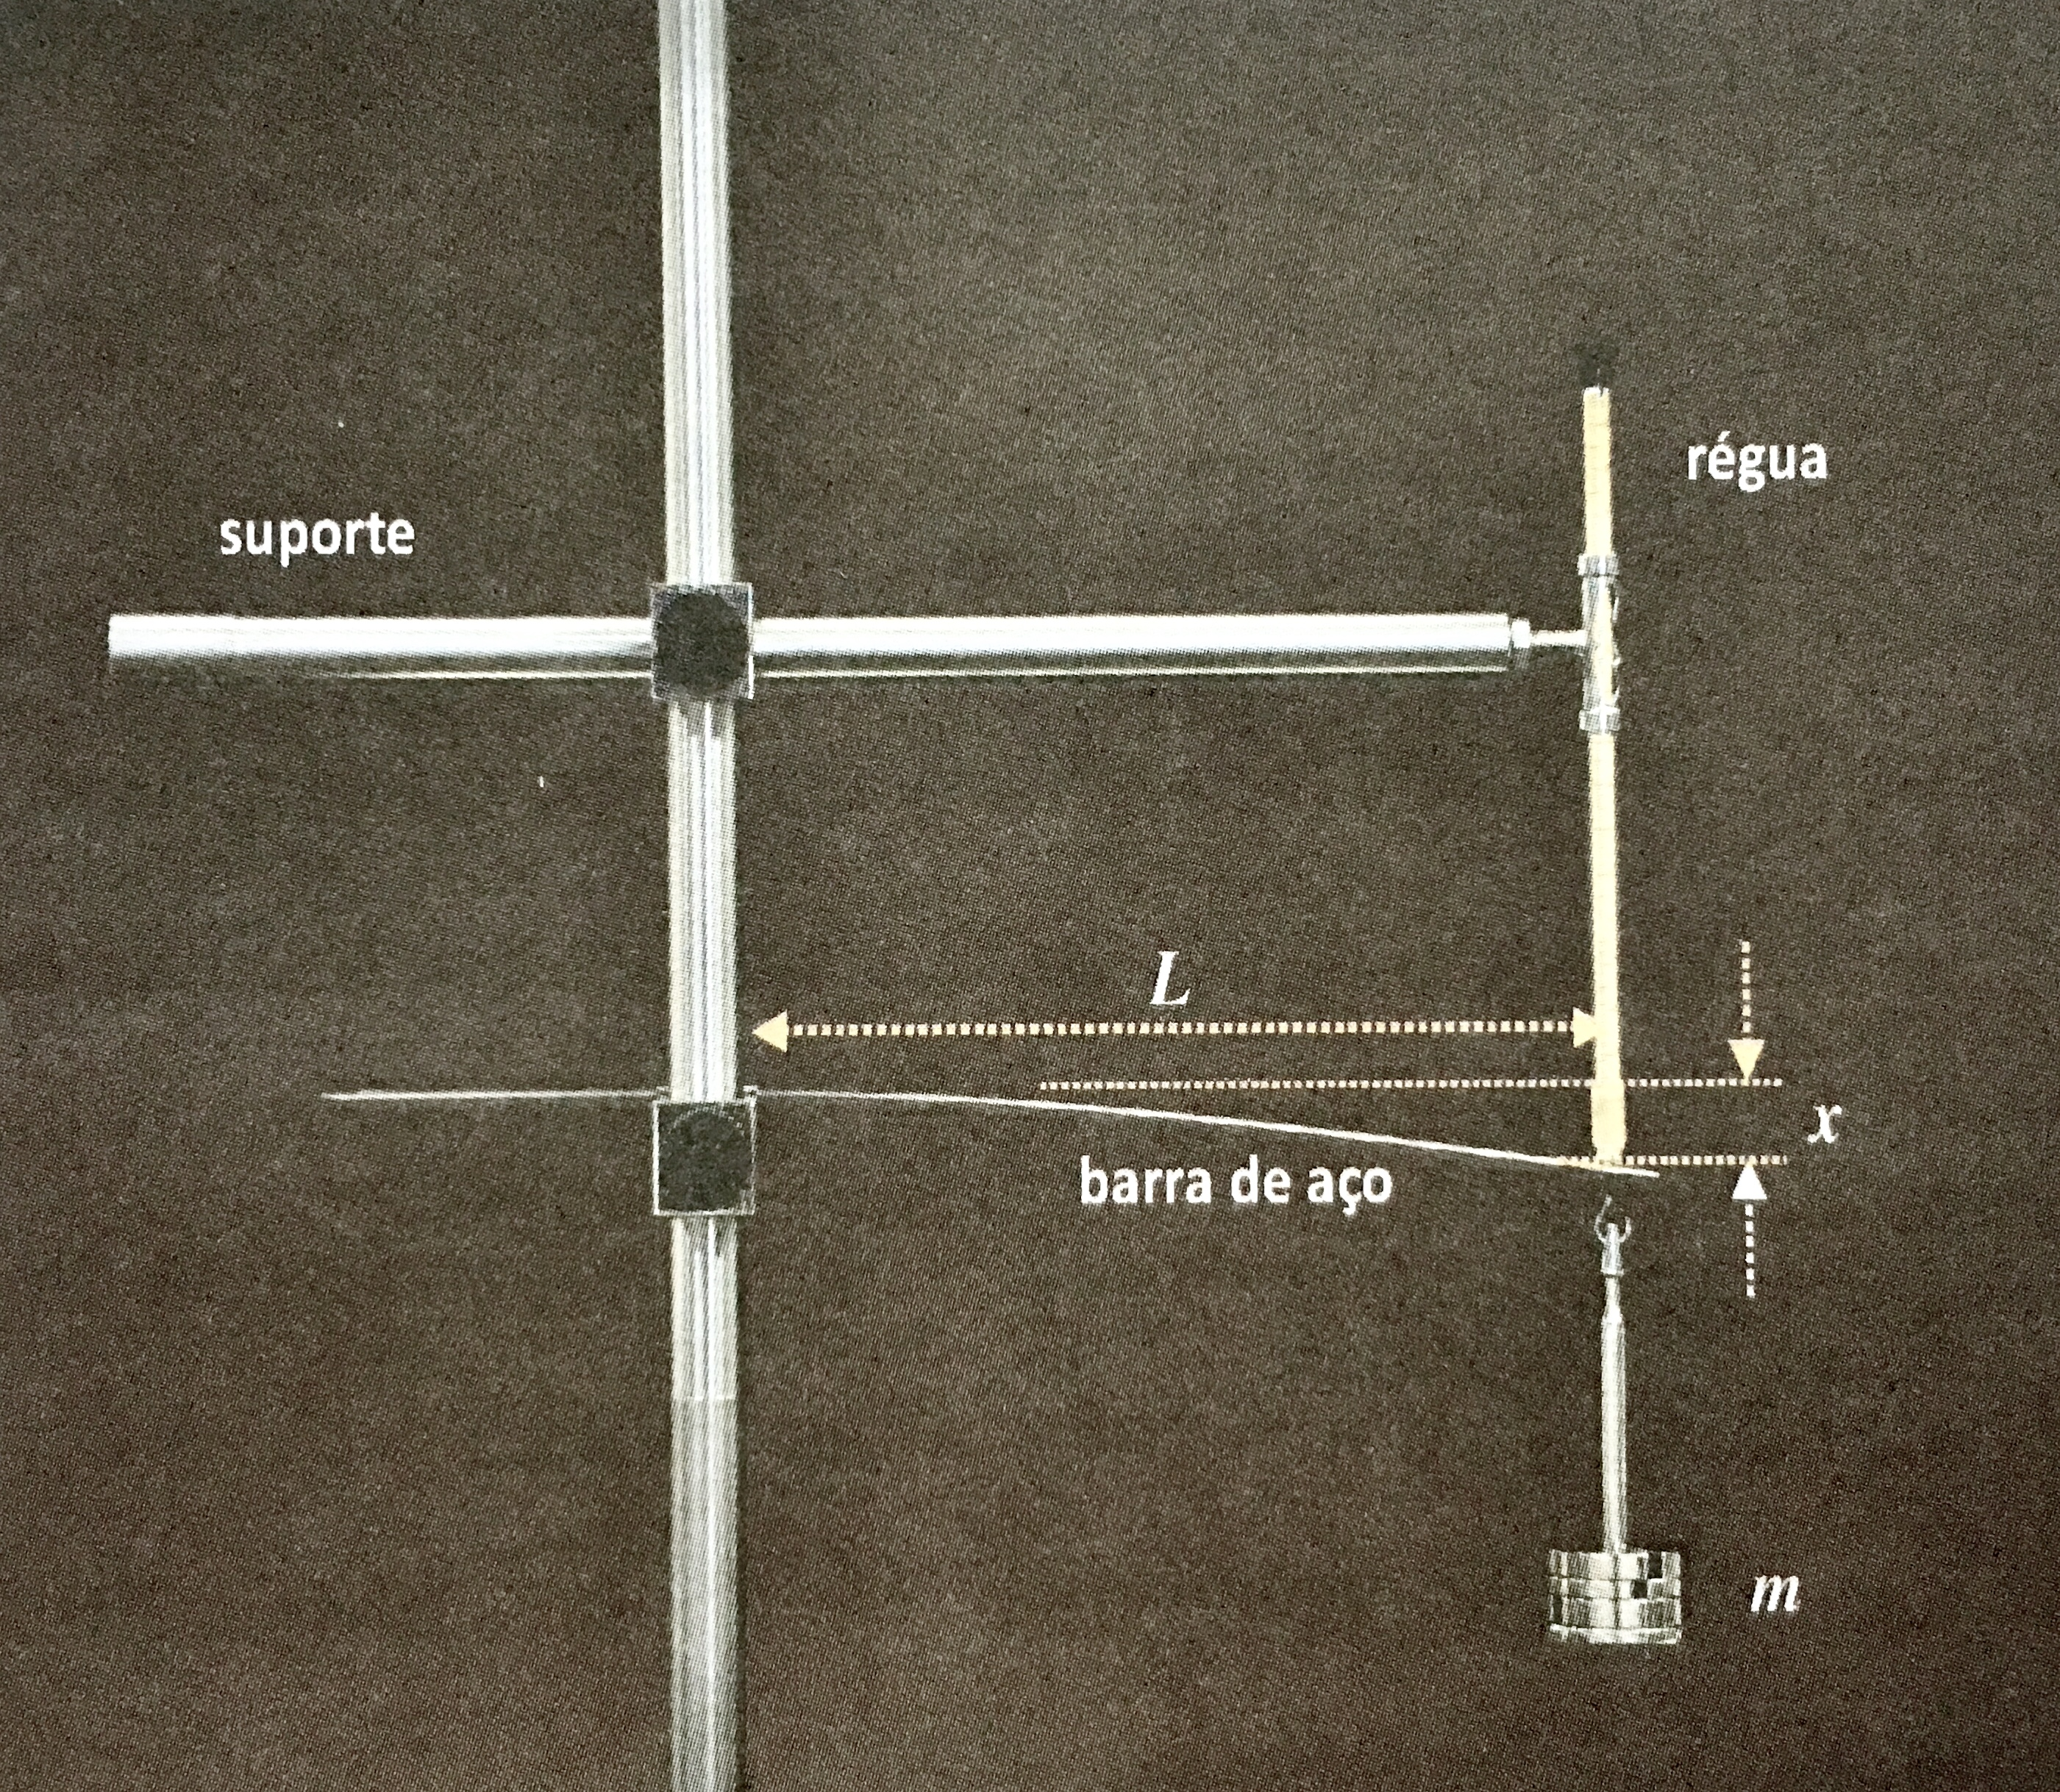
\includegraphics[width=0.5\textwidth]{IMG_1472.jpg}
\end{figure}

\begin{table}[!ht]
    \centering
    \caption{Aferições de massas e seus pesos}
    \label{tab:pesos}
    \begin{tabular}{c c|c|c}
        Ref. & Identificação & $Massa\pm 0.01\;(g)$ & $F_{peso}\pm0.000098\;(N)$ \\\hline
        $1:$ & $D1$ & $56.72$ & $0.555856$\\
        $2:$ & $D1 + D2$ & $109.80$ & $1.076040$\\
        $3:$ & $D1 + D2 + T4$ & $158.50$ & $1.553300$\\
        $4:$ & $D1 + D2 + T4 + D3$ & $209.47$ & $2.052806$\\
        $5:$ & $D1 + D2 + T4 + D3 + D4$ & $258.18$ & $2.530164$\\
        $6:$ & $D1 + D2 + T4 + D3 + D4 + D6$ & $302.88$ & $2.968224$\\
        $7:$ & $D1 + D2 + T4 + D3 + D4 + D6 + D9$ & $336.94$ & $3.302012$\\
        $8:$ & $D1 + D2 + T4 + D3 + D4 + D6 + D9 +T0$ & $383.94$ & $3.762612$\\
    \end{tabular}
\end{table}

\newpage
\subsection{Primeiro Procedimento: Diferentes pesos na extremidade da barra fixada à 27cm}

Dados:

$C\pm\sigma_C = (0.3\pm0.0005)\;m\;=$ comprimento e precisão do comprimento da barra;

$d\pm\sigma_d = (0.00098\pm0.00001)\;m\;=$ espessura e precisão da espessura da barra;

$b\pm\sigma_b = (0.025\pm0.00005)\;m\;=$ largura e precisão da largura da barra;

$l\pm\sigma_C = (0.27\pm0.0005)\;m\;=$ distenção e precisão do comprimento da barra como descrito na figura \ref{fig:disp};

$x_{i}\pm\sigma_x = (0.054\pm0.0005)\;m\;$ = comprimento inicial (deformação zero) e precisão da deformação.

Fixada uma barra à $l = 27\;cm$ no suporte para medições e alterando os pesos pendurados em sua extremidade (pesos referenciados na tabela \ref{tab:pesos}), medimos sua deformação $x$ em relação a altura original $x_i$ sem pesos.

\[\sigma_X^2 = \left(\frac{d(x-x_i)}{dx}\right)^2\cdot\sigma_x^2 + \left(\frac{d(x-x_i)}{dx_i}\right)^2\cdot\sigma_x^2\]
\[\sigma_X = \pm\sqrt{(1)^2\cdot25\cdot10^{-8} + (-1)^2\cdot25\cdot10^{-8}} = \pm\sqrt{5\cdot10^{-7}} = \pm0.0007071067811865475\;m\]

\begin{table}[!ht]
    \centering
    \caption{Aplicando-se diferentes pesos ($F_{peso}$), na mesma distancia ($l$), nota-se diferentes deformações ($(x - x_i)$).}
    \label{tab:p1}
    \begin{tabular}{c c|c|c}
        Peso Ref & $F_{peso}\pm\sigma_F\;(N)$ & $x\pm\sigma_x\;(m)$ & $(x - x_i)\pm\sigma_X\;(m)$\\
        \hline
        & sem pesos & $x_i = 0.054$ & $0.000$\\
        Ref. $1$ & $0.555856$ & $0.063$ & $0.009$\\
        Ref. $2$ & $1.076040$ & $0.071$ & $0.017$\\
        Ref. $3$ & $1.553300$ & $0.078$ & $0.024$\\
        Ref. $4$ & $2.052806$ & $0.086$ & $0.032$\\
        Ref. $5$ & $2.530164$ & $0.093$ & $0.039$\\
        Ref. $6$ & $2.968224$ & $0.100$ & $0.046$\\
        Ref. $7$ & $3.302012$ & $0.105$ & $0.051$\\
        Ref. $8$ & $3.762612$ & $0.112$ & $0.058$\\
    \end{tabular}
\end{table}


\begin{figure}[!ht]
    \centering
     \caption{Grafico de deformação $x - x_i$ pela força $F$ aplicada.}
    %\href{https://www.desmos.com/calculator/lwhpg1by6v}
    \label{gra:XxF}
    \includegraphics[width=0.4\textwidth]{XxF.png}
\end{figure}

%Utilizando dois pontos pertencentes à reta $(0.02, 1.29297128241)$ e $(0.05, 3.23242820601)$ obtemos o coeficiente angular.
Utilizando dois pontos pertencentes à reta $(0.02, 1.3829712824)$ e $(0.05, 3.23242820601)$ obtemos o coeficiente angular.



%\[k = \frac{\Delta y}{\Delta x} = \frac{3.23242820601-1.29297128241}{0.05-0.02} = 64.6485641203\]
\[k = \frac{\Delta y}{\Delta x} = \frac{3.23242820601-1.3829712824}{0.05-0.02} = 61.6485641203\]

Entao foi possivel calcular o Modulo de Young

%\[E = \frac{4l^3k}{d^3b} = \frac{4\cdot{0.27}^3\cdot64.6485641203}{{0.00098}^3\cdot0.025} = 21.631763765\cdot{10}^{10}\pm\sigma_E\;\left[N\cdot m^{-2}\right]\]
\[E = \frac{4l^3k}{d^3b} = \frac{4\cdot{0.27}^3\cdot61.6485641203}{{0.00098}^3\cdot0.025} = 20.627947328\cdot{10}^{10}\pm\sigma_E\;\left[N\cdot m^{-2}\right]\]
\[\sigma_E^2 = (\frac{dE}{dl})^2\sigma_l^2 + 
\left(\frac{dE}{dk}\right)^2\sigma_k^2 + 
\left(\frac{dE}{dd}\right)^2\sigma_d^2 + 
\left(\frac{dE}{db}\right)^2\sigma_b^2\]
\[\sigma_E = \pm\sqrt{
\left(\frac{12kl^2}{bd^3}\right)^2\cdot0.0005^2 +
\left(\frac{4l^3}{bd^3}\right)^2\cdot0^2 + 
\left(-\frac{12kl^3}{bd^4}\right)^2\cdot0.00001^2 + 
\left(-\frac{4kl^3}{d^3b^2}\right)^2\cdot0.00005^2
}\]
\[E = \left(20.627947328\pm0.67440253834\right)\cdot{10}^{10}\;\left[N\cdot m^{-2}\right]\]
\[E = \left(20.6\pm0.67\right)\cdot{10}^{10}\;\left[N\cdot m^{-2}\right]\]

Segundo a apostila esse modulo pertence ao material aço (Modulo de Young $= 20.0\times 10^{10} Pa$), portanto a barra em estudo é de aço.


\newpage
\subsection{Segundo Procedimento: Mesmo peso na extremidade da barra apoiada em pontos distintos}

Dados:

$C\pm\sigma_C = (0.3\pm0.0005)\;m\;=$ comprimento e precisão do comprimento da barra;

$d\pm\sigma_d = (0.00098\pm0.00001)\;m\;=$ espessura e precisão da espessura da barra;

$b\pm\sigma_b = (0.025\pm0.00005)\;m\;=$ largura e precisão da largura da barra;

$l\pm\sigma_C = (l\pm0.0005)\;m\;=$ distenção e precisão do comprimento da barra como descrito na figura \ref{fig:disp};

$x\pm\sigma_x = (x\pm0.0005)\;m\;$ = comprimento e precisão da deformação como descrito na figura \ref{fig:disp}.

Fixado o peso Ref. 7 na extremidade da barra movendo-a no suporte para medições, medimos sua deformação $x$.

\[\sigma_{l^{3}}^2 = \left(\frac{d(l^3)}{dl}\right)^2\sigma_C^2\]
\[\sigma_{l^{3}} = \pm\sqrt{\left(3l^2\right)^2\cdot\sigma_C^2} = \pm0.0015l^2\]

\begin{table}[!ht]
    \centering
    \caption{Em diferentes comprimentos ($l$), com o mesmo peso ($P = 3.302012\;N$), observa-se diferentes deflexões ($x_f - x_i$).}
    \label{tab:p2}
    \begin{tabular}{c|c|c|c|c}
        $l\pm\sigma_C\;(m)$ & $l^3\pm\sigma_{l^3}\;(m^3)$ & $x_f\pm\sigma_{x_f}\;(m)$ & $x_i\pm\sigma_{x_i}\;(m)$ & $(x_f - x_i)\pm\sigma_X\;(m)$\\\hline
        $0.270$ & $0.019683$ & $0.105$ & $0.054$ & $0.051$\\
        $0.250$ & $0.015625$ & $0.096$ & $0.052$ & $0.044$\\
        $0.230$ & $0.012167$ & $0.085$ & $0.051$ & $0.034$\\
        $0.210$ & $0.009261$ & $0.077$ & $0.050$ & $0.027$\\
        $0.190$ & $0.006859$ & $0.070$ & $0.050$ & $0.020$\\
        $0.170$ & $0.004913$ & $0.064$ & $0.050$ & $0.014$\\
        $0.150$ & $0.003375$ & $0.059$ & $0.050$ & $0.009$\\
        $0.130$ & $0.002197$ & $0.056$ & $0.050$ & $0.006$\\
        $0.110$ & $0.001331$ & $0.054$ & $0.050$ & $0.004$\\
        $0.090$ & $0.000729$ & $0.052$ & $0.050$ & $0.002$\\
        $0.070$ & $0.000343$ & $0.050$ & $0.049$ & $0.001$\\
    \end{tabular}
\end{table}

\[P = \frac{Ed^3b}{4l^3}x\]
\[x(l) = \left(\frac{4P}{Ed^3b}\right)l^3\]
\[A = \frac{4P}{Ed^3b}\]
\[x = (A)l^3\]
\[\log{x} = \log{A} + 3\log{l}\]
Pegando dois pontos pertencentes á reta e aplicando a funcao $\log$ é possivel encontrar um valor proximo à $3$, como esperado por ser uma função cubica (coeficiente $3$ na equação acima).
\[k = \frac{\log{x_2}-\log{x_1}}{\log{l_2}-\log{l_1}} = \frac{\log{0.034}-\log{0.001}}{\log{0.230}-\log{0.070}} = 2.96436428733\pm\sigma_{k}\]
%\[\log_{\left(\frac{0.230}{0.070}\right)}{\left(\frac{0.034}{0.001}\right)}\]
%\left(\right)
\[\sigma_k^2 = \left(\frac{dk}{dx_2}\right)^2\sigma_{x_2}^2 + \left(\frac{dk}{dx_1}\right)^2\sigma_{x_1}^2 + \left(\frac{dk}{dl_2}\right)^2\sigma_{l_2}^2 + \left(\frac{dk}{dl_1}\right)^2\sigma_{l_1}^2\]
%\[\sigma_k^2 = \left(\frac{1}{x_2(\ln{l_2}-\ln{l_1})}\right)^2\sigma_{x_2}^2 + \left(\frac{-1}{x_1(\ln{l_2}-\ln{l_1})}\right)^2\sigma_{x_1}^2 + \left(\frac{\ln{x_1}-\ln{x_2}}{l_2(\ln{l_2}-\ln{l_1})^2}\right)^2\sigma_{l_2}^2 + \left(\frac{\ln{x_2}-\ln{x_1}}{l_1(\ln{l_2}-\ln{l_1})^2}\right)^2\sigma_{l_1}^2\]
\[\sigma_k = 0.420908153691\]
\[k = 2.96436428733\pm0.420908153691\]
\[k = 3.0\pm0.4\]
Agora procuraremos $A$ para depois encontrarmos o modulo de Young:
\[A = \frac{x_2-x_1}{l_2^3-l_1^3} = \frac{0.034-0.001}{0.230^3-0.070^3} = 2.79093369418\pm\sigma_A\]
\[\sigma_A^2 = \left(\frac{dA}{dx_2}\right)^2\sigma_{x_2}^2 + \left(\frac{dA}{dx_1}\right)^2\sigma_{x_1}^2 + \left(\frac{dA}{dl_2}\right)^2\sigma_{l_2}^2 + \left(\frac{dA}{dl_1}\right)^2\sigma_{l_1}^2\]
\[\sigma_A^2 = \left(\frac{1}{l_2^3-l_1^3}\right)^2\sigma_{x_2}^2 + \left(\frac{-1}{l_2^3-l_1^3}\right)^2\sigma_{x_1}^2 + \left(\frac{\ln{x_1}-\ln{x_2}}{l_2(\ln{l_2}-\ln{l_1})^2}\right)^2\sigma_{l_2}^2 + \left(\frac{\ln{x_2}-\ln{x_1}}{l_1(\ln{l_2}-\ln{l_1})^2}\right)^2\sigma_{l_1}^2\]
\[E = \frac{4P}{Ad^3b} = \frac{4\cdot3.302012}{2.79093369418\cdot0.00098^3\cdot0.025} = 20.112723537\cdot{10}^{10}\;\left[N\cdot m^{-2}\right]\]


\begin{figure}[!ht]
    \centering
     \caption{Grafico de deformação $x_f - x_i$ pelo comprimento $l^3$.}
    %\href{https://www.desmos.com/calculator/vz1ffqbye1}
    \label{gra:XxL}
    \includegraphics[width=0.4\textwidth]{XxL.png}
\end{figure}



\section{Resultados e discussão}

\indent

As contas bateram com a literatura nas duas abordagens

\end{document}
